%% ===========================================================================
%% DRAFT 2 -- structured to the course content template, typeset with the
%% IEEE Access class (ieeeaccess.cls on top of IEEEtran.cls).
%% Every number in this file is produced by the scripts in ../paper_eval/.
%% Data-table rows are read from ./tables/ (generated); figures from ./figures/.
%% ===========================================================================
\documentclass{ieeeaccess}
\usepackage{cite}
\usepackage{amsmath,amssymb,amsfonts}
\usepackage{algorithmic}
\usepackage{algorithm}
\usepackage{graphicx}
\usepackage{textcomp}
\usepackage{booktabs}
\usepackage{multirow}
\usepackage{array}
\usepackage{url}

\newcommand{\clir}{CLIR}
% Rows of the data tables are generated by paper_eval/make_tables.py.
% TeX's primitive \input is used so that the rows can be read inside a tabular.
\makeatletter
\newcommand{\rowsfrom}[1]{\@@input #1 }
\makeatother
% ieeeaccess.cls formats a caption according to \xfigwd, which only its own
% \Figure macro sets; with the standard figure environments used here, 0pt
% selects the class's normal (wrapping) caption style.
\gdef\xfigwd{0pt}
\renewcommand{\algorithmicrequire}{\textbf{Input:}}
\renewcommand{\algorithmicensure}{\textbf{Output:}}

\begin{document}
\history{Date of publication xxxx 00, 0000, date of current version xxxx 00, 0000.}
\doi{10.1109/ACCESS.2017.DOI}

\title{Optimize Before You Compress: SSA-Based Compaction of Three-Address Code, Verified by Differential Testing}

%% Authors: Team 16, Hrituraj Deb first (requested), then as on the team list.
\author{\uppercase{Hrituraj Deb}\authorrefmark{1},
\uppercase{Gautham G}\authorrefmark{1},
\uppercase{Rishabh Kumar}\authorrefmark{1}, and
\uppercase{Aarnav Bhasin}\authorrefmark{1}}
\address[1]{School of Computer Science and Engineering, Vellore Institute of Technology, Vellore 632014, India (e-mail: hrituraj.deb2024@vitstudent.ac.in; gautham.g2024@vitstudent.ac.in; rishabh.kumar2024@vitstudent.ac.in; aarnav.bhasin2024@vitstudent.ac.in)}
\tfootnote{This work received no external funding.}

\markboth
{H. Deb \headeretal: Optimize Before You Compress: SSA-Based Compaction of Three-Address Code}
{H. Deb \headeretal: Optimize Before You Compress: SSA-Based Compaction of Three-Address Code}

\corresp{Corresponding author: Hrituraj Deb (e-mail: hrituraj.deb2024@vitstudent.ac.in).}

\begin{abstract}
Software increasingly reaches phones, browsers and embedded devices as portable intermediate code rather than as native binaries. Every byte costs download time, flash storage and memory. Small programs, such as plug-ins and over-the-air updates, are the common case. Compilers lower source programs to three-address code, which is verbose: literals sit in fresh temporaries, values are recomputed, and dead branches survive. Tools often report size savings without saying whether optimization or encoding produced them. Existing work shrinks programs with compiler transformations such as function merging, loop rolling, outlining and machine-learned pass ordering. Other work stores intermediate code as a file and compresses it with Brotli, Zstandard or xz. The first group targets native binaries in large production toolchains. The second is blind to program semantics and pays a fixed cost per file. We present a pipeline that converts three-address code to static single assignment form, runs five optimization passes to a fixed point and writes the result as a compact bytecode with variable-length operands. Every number is verified by independent decoders, reference interpreters and differential testing. On seven benchmarks, optimization removed 18.5\% to 89.3\% of the instructions. The bytecode was 68.7\% to 87.8\% smaller than the textual code and 37.3\% to 75.4\% smaller than the best of the three compressors applied to that text. Huffman coding helped only above about 5.7 kilobytes. Differential testing on 1000 programs exposed one folding defect, and its fix was confirmed. Future work will add copy propagation, a self-describing bytecode and real C benchmark suites.
\end{abstract}

\begin{keywords}
Bytecode compression, compiler optimization, differential testing, Huffman coding, intermediate representation, static single assignment.
\end{keywords}

\titlepgskip=-15pt

\maketitle

%% ===========================================================================
\section{Introduction}
\label{sec:introduction}
%% ===========================================================================
\PARstart{P}{ortable} intermediate code has become a common way to deliver software. Embedded and Internet of Things (IoT) devices receive new functionality through over-the-air updates, where every transmitted byte costs radio energy and every stored byte costs flash memory~\cite{bauwens2020ota}. Web browsers execute WebAssembly modules, a standardized portable bytecode~\cite{w3c2019wasm}, whose performance and deployment have been studied on large application suites~\cite{jangda2019wasm}. Compiler infrastructures such as MLIR keep programs in several levels of intermediate representation (IR) before any machine code is produced~\cite{lattner2021mlir}. Most of these representations build on static single assignment (SSA) form, in which every variable is defined exactly once~\cite{rastello2022ssa}.

The problem studied in this article is the size of such intermediate code when it must be stored or sent. A straightforward lowering of a C-like program to three-address code (TAC) is verbose. Every literal is placed in a fresh temporary, expressions whose operands are compile-time constants are left for run time, and branches that can never be taken are kept. Our motivation is practical. A teaching compiler built by our team, called IR (intermediate representation) Compression Studio, reported large end-to-end savings, but it was unclear how much of each saving came from optimization, how much from the binary format, and whether every reported number and every optimization was correct. Small programs make the question sharper, because fixed per-file costs such as coder tables can outweigh the payload.

Existing methodologies attack program size from two directions. The first direction transforms the program. Classic scalar optimizations such as constant propagation, value numbering and dead-code elimination are textbook material~\cite{cooper2022eac}, and SSA form makes them sparse and fast~\cite{rastello2022ssa}. Production compilers add size-specific transformations and increasingly choose among them with machine learning~\cite{wang2018ml,ashouri2018autotuning}.

The second direction encodes the program compactly after it has been produced. Entropy coders such as Huffman codes assign short bit strings to frequent symbols and are still widely used inside larger compressors~\cite{moffat2019huffman}. General-purpose compressors combine such coders with string matching and can be applied to any IR file without knowing what it contains.

Both directions have shortfalls for small intermediate programs. Size-oriented compiler transformations, such as function merging, loop rolling, inlining and outlining~\cite{rocha2020salssa,rocha2021hyfm,rocha2022rolag,damasio2021inlining,theodoridis2022inlining,chabbi2021ios}, are built into large production toolchains and are evaluated on native binaries of whole applications, so their gains are hard to reproduce in a small educational compiler or to separate from the binary format. Machine-learned approaches~\cite{trofin2021mlgo,jain2022posetrl,cummins2023llm,cummins2021compilergym,cummins2021programl} add training infrastructure and models that are larger than the programs they optimize.

General-purpose compressors are blind to program semantics. They cannot remove an instruction that is never executed, and on inputs of a few hundred bytes their containers and coding tables are a large fraction of the output. Neither direction routinely checks that the transformed program still behaves like the original, although compilers are known to contain miscompilation bugs that only systematic testing reveals~\cite{chen2020testing}.

This article proposes an SSA-based compaction pipeline that optimizes first and encodes second. The program is lowered to TAC, converted to semi-pruned SSA form and optimized with five passes iterated to a fixed point: constant folding and propagation, dominator-scoped value numbering, dead-code elimination, CFG simplification and trivial-$\phi$ removal. The optimized code is then written as a compact bytecode, which we call \clir{}, using one opcode byte and Little Endian Base 128 (LEB128) operands~\cite{w3c2019wasm}, optionally followed by a static Huffman coder or a column-oriented container. The approach is apt because the programs are small and their values are often known at compile time, which is exactly where removing instructions beats compressing them.

The main advantage of the proposed work is that its claims are checked rather than assumed. Every number the pipeline reports is recomputed by independent scripts. The byte streams are decoded by a parser written from the format description alone. Behavior is compared by reference interpreters on 1000 random programs, and a two-parameter model explains when entropy coding starts to pay off. The contributions are: 1) a reproducible SSA compaction pipeline with an exact byte layout; 2) an evaluation on seven benchmarks and 1264 synthetic programs, with a comparison against Brotli, Zstandard and xz; 3) a break-even model for static Huffman coding; and 4) a differential-testing campaign that found and confirmed a fix for a constant-folding defect.

The rest of the manuscript is structured as follows. Section~\ref{sec:related} reviews fifteen related works. Section~\ref{sec:proposed} formulates the problem and presents the architecture, methodology, modules, flow, equations and algorithms of the proposed system. Section~\ref{sec:results} describes the implementation tools, parameter setup and performance metrics, and analyzes the results against existing compressors. Section~\ref{sec:conclusion} concludes and outlines future work.

%% ===========================================================================
\section{Related Works}
\label{sec:related}
%% ===========================================================================
This section reviews fifteen recent works in four groups: compiler transformations that reduce code size, machine-learning-guided optimization, studies of portable bytecode, and compiler correctness. For each work we summarize the proposed solution, the methodology and tools, the results, and the research gap that remains for compact intermediate code. Table~\ref{tab:related} gives an overview.

\subsection{Code-Size Reduction by Compiler Transformations}

\subsubsection{SalSSA, function merging in SSA form}
\textit{Solution.} Rocha \textit{et al.}~\cite{rocha2020salssa} proposed SalSSA, which merges similar functions into one while staying in SSA form, so that the register demotion required by the earlier FMSA approach is no longer needed. The merged control-flow graph is built top-down from the two input graphs, and a $\phi$-node coalescing step reduces the extra code that merging introduces.

\textit{Methodology and tools.} Each function is linearized into labels and instructions, and a sequence alignment pairs matching instructions. $\phi$-nodes travel with their block labels, mismatched operands are chosen with a \texttt{select} on a function identifier, and the operands of commutative instructions are reordered to avoid selects.

SalSSA was implemented in LLVM 11 and evaluated on SPEC CPU2006 and CPU2017 on an Intel x86 machine, and on MiBench for ARM Thumb, against FMSA. Object size, compile time, peak memory and run time were measured over five repetitions.

\textit{Results.} Code size fell by 9.3\% to 9.7\% on SPEC CPU2006 and 7.9\% to 9.2\% on CPU2017, about twice the reduction of FMSA. Compile-time overhead was about 5\% instead of 14\%, and memory use roughly halved.

\textit{Research gap.} The work targets whole functions in native binaries; it does not consider how the remaining IR is encoded.

\subsubsection{HyFM, hybrid function merging}
\textit{Solution.} HyFM~\cite{rocha2021hyfm} aligns functions block by block instead of as whole instruction sequences. A multi-tier profitability analysis discards unprofitable block pairs before any merged code is generated.

\textit{Methodology and tools.} Blocks and functions are summarized by vectors of opcode counts, paired by Manhattan distance, and aligned either with the Needleman--Wunsch algorithm or with a linear pairwise alignment of equal-sized blocks. The first tier compares the estimated cost of each block pair before and after merging.

HyFM was implemented in LLVM 11, the same version as SalSSA, and evaluated on SPEC CPU2006 and CPU2017 on an Intel Xeon machine with five repetitions. Code size, merging time, compile time and peak memory were reported.

\textit{Results.} With pairwise alignment, the code-size reduction stayed within one percentage point of SalSSA, while function merging ran 4.59 to 5.28 times faster on average and peak memory dropped from 2.4~GB to about 610~KB.

\textit{Research gap.} Block pairing is still quadratic in the number of blocks, and the work remains specific to native code.

\subsubsection{RoLAG, loop rolling}
\textit{Solution.} RoLAG~\cite{rocha2022rolag} rolls isomorphic straight-line code back into loops. It finds repeated code by aligning SSA graphs bottom-up from seed instructions such as stores and calls.

\textit{Methodology and tools.} Mismatching values become loop inputs, and special patterns such as monotonic integer sequences, chained dependences and reduction trees widen the code that can be aligned. A scheduling analysis checks that reordering is legal, and a profitability analysis based on LLVM's code-size cost model keeps the smaller version.

RoLAG was built on LLVM 12 and evaluated with \texttt{-Os} on about one million AnghaBench functions, on MiBench and SPEC CPU2017 programs, and on the TSVC kernels, against LLVM's loop-rerolling pass.

\textit{Results.} Affected AnghaBench functions shrank by 9.12\% on average, and the largest absolute saving on full programs was 87.91~KB. On TSVC, RoLAG reduced size by 23.4\% against 13.69\% for LLVM.

\textit{Research gap.} Rolling works only inside a single basic block and can be unprofitable when the cost model misses later passes.

\subsubsection{Inlining for code size}
\textit{Solution.} Dam\'asio \textit{et al.}~\cite{damasio2021inlining} showed that inlining, usually seen as a code-growing transformation, can shrink code. They inline functions that have a single call site and then delete the original, and they search for calls at which inlining lets the compiler simplify the body for that particular caller.

\textit{Methodology and tools.} The first technique is a simple heuristic over the call graph. The second is an analysis that estimates whether specializing the callee to the constants at a call site will remove code.

Both techniques were implemented in LLVM and evaluated on MiBench against \texttt{clang -Os}, with running time compared statistically.

\textit{Results.} Code size fell by 2.96\% on average and by up to 11\%, with no statistically significant change in running time.

\textit{Research gap.} The evaluation covers one benchmark suite and native code only.

\subsubsection{Optimal function inlining}
\textit{Solution.} Theodoridis \textit{et al.}~\cite{theodoridis2022inlining} studied how far LLVM's inliner is from optimal when optimizing for binary size and derived an autotuning strategy from the findings.

\textit{Methodology and tools.} A formulation of the inlining problem shrinks the search space enough to evaluate every inlining choice exhaustively for 1135 SPEC2017 files.

The autotuner was then applied to SPEC2017, the LLVM code base and SQLite, with LLVM's heuristic as the baseline.

\textit{Results.} The authors report an average improvement of 7\% (up to 28\%) over LLVM on SPEC2017, 15\% on LLVM's own code and 10\% on SQLite.

\textit{Research gap.} The study focuses on one transformation in a production compiler and does not address the encoding of portable code.

\subsubsection{Code-size optimization of production iOS applications}
\textit{Solution.} Chabbi \textit{et al.}~\cite{chabbi2021ios} reduced the size of a production iOS application written in Swift and Objective-C with whole-program machine-code outlining, repeated over several rounds.

\textit{Methodology and tools.} An analysis pass logged repeated instruction sequences and traced them to causes such as reference-counting calls, frame setup and copies produced when leaving SSA form.

All modules were compiled to LLVM IR, linked with \texttt{llvm-link}, optimized and then outlined as one program, using Swift 5.2, Xcode and patched LLVM for AArch64 devices, with production data from millions of users.

\textit{Results.} The code section of the UberRider application shrank by 23\% (114.5~MB to 88.4~MB) and the whole binary by 17.6\%; the Linux kernel and Clang shrank by 14\% and 25\%. Release builds took 66 instead of 21 minutes.

\textit{Research gap.} The approach needs a custom toolchain and much longer builds, and it works on machine code rather than on portable IR.

\subsection{Machine-Learning-Guided Optimization}

\subsubsection{MLGO}
\textit{Solution.} MLGO~\cite{trofin2021mlgo} is a framework for using machine-learned policies inside LLVM. Its first application replaces the heuristic in LLVM's inlining-for-size pass.

\textit{Methodology and tools.} Inlining is modeled as a sequential decision process with eleven numerical features of caller, callee and call graph. Policies are trained with policy gradient, warm-started by imitating the existing heuristic, and with evolution strategies.

Training used TF-Agents on more than 28,000 IR modules of an internal application, and the released model is compiled ahead of time into LLVM, so that compilation stays deterministic.

\textit{Results.} The learned policies reduced size by up to 7\% compared with \texttt{-Oz}, for about 1\% extra compile time.

\textit{Research gap.} The method needs large training infrastructure and targets native size only.

\subsubsection{POSET-RL}
\textit{Solution.} POSET-RL~\cite{jain2022posetrl} uses reinforcement learning to choose the order of optimization passes so that code size and execution time both improve.

\textit{Methodology and tools.} A Double Deep Q-Network observes 300-dimensional IR2Vec embeddings of the program and selects sub-sequences of the \texttt{-Oz} pipeline. These come from a manual grouping or from an Oz Dependence Graph. The reward combines object-size reduction with throughput estimated by LLVM-MCA.

The agent was trained in LLVM 10 on 130 files from the LLVM test suite and evaluated on MiBench, SPEC CPU2006 and SPEC CPU2017 on x86 and AArch64.

\textit{Results.} The graph-based variant improved code size by 6.19\% and execution time by 11.99\% over \texttt{-Oz} on SPEC CPU2017 on average.

\textit{Research gap.} The rewards are proxies, and some benchmarks grew or slowed down.

\subsubsection{Large language models for compiler optimization}
\textit{Solution.} Cummins \textit{et al.}~\cite{cummins2023llm} trained a 7-billion-parameter transformer to read unoptimized LLVM IR and emit a list of passes that minimizes the instruction count.

\textit{Methodology and tools.} The model follows the Llama~2 architecture and was trained from scratch on one million LLVM-IR functions (about 373 million tokens). Auxiliary tasks ask it to predict instruction counts and the optimized code.

Training labels came from an autotuner that ran tens of thousands of compilations per program. Evaluation used 100,000 unseen functions and compared the model with AutoPhase and Coreset-NVP.

\textit{Results.} The model's pass lists produced 3.01\% fewer instructions than \texttt{-Oz} without extra compilations, and its generated code compiled 90.3\% of the time.

\textit{Research gap.} The model cannot reliably fold constants, its context is limited to 2048 tokens, and inference is far slower than compilation.

\subsubsection{CompilerGym}
\textit{Solution.} CompilerGym~\cite{cummins2021compilergym} packages compiler optimization tasks as reinforcement-learning environments with the OpenAI Gym interface.

\textit{Methodology and tools.} A Python front end talks to compiler services over remote procedure calls. Environments cover LLVM phase ordering with 124 passes, GCC flag tuning and CUDA loop nests. Observations range from instruction counts to graph representations, and rewards include IR instruction count relative to \texttt{-Oz}.

More than one million LLVM benchmarks are bundled, and the framework validates semantics with differential testing and sanitizers.

\textit{Results.} An environment step took 7.5~ms instead of 205.9~ms in earlier work, about 27 times faster. The best autotuner reached 1.083 times the code-size reduction of \texttt{-Oz} on cBench.

\textit{Research gap.} It is an experimentation platform, and its learning agents generalized poorly across program domains.

\subsubsection{ProGraML}
\textit{Solution.} ProGraML~\cite{cummins2021programl} is a language-independent graph representation of programs for machine learning, combining control, data and call relations in one multigraph.

\textit{Methodology and tools.} Instructions, identifiers and immediate values become vertices built from LLVM or XLA IR, with typed and ordered edges. A message-passing neural network learns over the graph.

Classic data-flow analyses such as reachability, dominators and liveness were posed as supervised learning tasks on a large dataset of IR files, and the representation was then applied to downstream optimization tasks.

\textit{Results.} The authors found that earlier learned representations struggle to reproduce data-flow analyses and that ProGraML improves results on downstream tasks.

\textit{Research gap.} It learns analyses that a compiler can compute exactly, and it does not produce compact program encodings.

\subsection{Studies of Portable Bytecode}

\subsubsection{Real-world WebAssembly binaries}
\textit{Solution.} Hilbig \textit{et al.}~\cite{hilbig2021wasm} conducted a large empirical study of WebAssembly binaries found in the wild.

\textit{Methodology and tools.} The authors collected 8461 unique binaries from source repositories, package managers and live websites.

They analyzed source languages, security-relevant imports and use cases, and released the collection, 58 times the size of any WebAssembly benchmark used before.

\textit{Results.} Two thirds of the binaries were compiled from memory-unsafe languages, 21\% imported potentially dangerous host functions, and 29\% of the binaries on websites were minified.

\textit{Research gap.} The study characterizes binaries but does not try to make them smaller.

\subsubsection{Superoptimization of WebAssembly bytecode}
\textit{Solution.} Cabrera Arteaga \textit{et al.}~\cite{cabrera2020superopt} superoptimized WebAssembly code by inserting the Souper superoptimizer into an LLVM-to-WebAssembly pipeline.

\textit{Methodology and tools.} C programs were compiled with Clang at \texttt{-O3} to LLVM bitcode, passed through Souper, which proves replacements equivalent with an SMT solver, and linked to WebAssembly.

Four Souper configurations with a 300-second timeout were tried on 12 Rosetta Code programs, and the instruction counts of the resulting modules were compared.

\textit{Results.} The median reduction was 0.33\% of the instructions. One program shrank from 45 to 21 instructions, and one program grew.

\textit{Research gap.} The cost model works on LLVM IR rather than on the final bytecode, and the evaluation is small.

\subsection{Compiler Correctness}

\subsubsection{Alive2}
\textit{Solution.} Alive2~\cite{lopes2021alive2} checks automatically, without changes to LLVM, that each optimized function refines the original one, a technique known as translation validation.

\textit{Methodology and tools.} Source and target functions are encoded for the Z3 SMT solver with LLVM's forms of undefined behavior. Loops are unrolled to a bound, which keeps checking fast but means some bugs are missed.

The tool was run over the functions in LLVM's unit-test suite that exercise IR-level transformations.

\textit{Results.} The tool exposed 47 previously unknown bugs, of which 28 had been fixed at the time of writing, and led to eight corrections of the LLVM language reference.

\textit{Research gap.} The approach depends on a full formal semantics of the IR and on a solver, which a small compiler does not have.

\subsubsection{YARPGen}
\textit{Solution.} YARPGen~\cite{livinskii2020yarpgen} generates random C and C++ programs that are free of undefined behavior and uses them for differential testing of compilers.

\textit{Methodology and tools.} The generator tracks values while generating and rewrites operations that could trigger undefined behavior; the rewrite rules were checked exhaustively on 4-bit values and with Z3.

Generation policies steer programs toward patterns that trigger specific optimizations. The compilers under test were GCC, LLVM and Intel's C++ compiler, all targeting x86-64.

\textit{Results.} YARPGen found 83 new bugs in GCC, 62 in LLVM and 76 in the Intel compiler, and its policies triggered targeted optimizations 20\% (LLVM) and 40\% (GCC) more often.

\textit{Research gap.} It tests production C compilers, not the compactness or losslessness of IR encodings.

\begin{table*}[!t]
\centering
\caption{Summary of the related works reviewed in Section~\ref{sec:related}}
\label{tab:related}
\footnotesize
\setlength{\tabcolsep}{3pt}
\begin{tabular}{@{}p{23mm} p{38mm} p{37mm} p{35mm} p{33mm}@{}}
\toprule
Work & Technique & Tools and benchmarks & Reported result & Gap for compact IR \\
\midrule
SalSSA~\cite{rocha2020salssa} & Function merging in SSA form & LLVM 11; SPEC CPU2006/2017, MiBench & 7.9--9.7\% smaller code & Native code; no encoding \\
HyFM~\cite{rocha2021hyfm} & Block-level function merging & LLVM 11; SPEC CPU2006/2017 & Merging 4.59--5.28$\times$ faster & Quadratic pairing; native \\
RoLAG~\cite{rocha2022rolag} & Loop rolling by SSA graph alignment & LLVM 12; AnghaBench, SPEC, TSVC & 9.12\% on affected functions & Single block only \\
Inlining~\cite{damasio2021inlining} & Size-reducing inlining heuristics & LLVM; MiBench & 2.96\% average, up to 11\% & One suite, native \\
Optimal inlining~\cite{theodoridis2022inlining} & Exhaustive study and autotuning & LLVM; SPEC2017, SQLite & 7\% average over LLVM & One transformation \\
iOS outlining~\cite{chabbi2021ios} & Repeated whole-program outlining & Swift, LLVM, AArch64 & 23\% smaller code section & Custom toolchain \\
MLGO~\cite{trofin2021mlgo} & Learned inlining policy & LLVM, TF-Agents & Up to 7\% vs \texttt{-Oz} & Training cost \\
POSET-RL~\cite{jain2022posetrl} & RL pass ordering & LLVM 10, IR2Vec; SPEC, MiBench & 6.19\% size, SPEC2017 & Proxy rewards \\
LLM~\cite{cummins2023llm} & 7B transformer picks passes & LLVM 10; 100k test functions & 3.01\% fewer instructions & No constant folding \\
CompilerGym~\cite{cummins2021compilergym} & Gym environments & LLVM, GCC, CUDA & 27$\times$ faster steps & Platform only \\
ProGraML~\cite{cummins2021programl} & Program graphs for ML & LLVM, XLA; MPNN & Better downstream tasks & Learns exact analyses \\
Wasm study~\cite{hilbig2021wasm} & Empirical study of binaries & 8461 binaries & 29\% of web binaries minified & No size reduction \\
Wasm superopt.~\cite{cabrera2020superopt} & Souper on LLVM to Wasm & 12 Rosetta Code programs & 0.33\% median reduction & IR-level cost model \\
Alive2~\cite{lopes2021alive2} & Translation validation & Z3; LLVM unit tests & 47 new bugs & Needs formal IR semantics \\
YARPGen~\cite{livinskii2020yarpgen} & UB-free random programs & GCC, LLVM, ICC & 221 new bugs & Tests compilers, not encodings \\
\bottomrule
\end{tabular}
\end{table*}

\subsection{Summary of the Research Gap}
The reviewed works either transform native code inside large production toolchains, learn optimization policies with substantial infrastructure, study bytecode without shrinking it, or test compilers without looking at encodings. None of them measures, at the level of a small IR, how much of a size reduction comes from optimization and how much from the binary format, or compares such a pipeline with general-purpose compressors while checking that program behavior is preserved. The proposed work addresses this combination.

%% ===========================================================================
\section{Proposed Work and System}
\label{sec:proposed}
%% ===========================================================================
\subsection{Problem Formulation}
Let $P$ be a source program and $T=\langle t_1,\dots,t_n\rangle$ the three-address code produced for it. The observable behavior $\mathrm{Obs}(T)$ is the sequence of printed values together with the returned value. The goal is to find an optimized instruction list $T^\ast$ and an encoding $E$ that minimize the encoded size while keeping the behavior and allowing the instructions to be decoded:
\begin{equation}
\begin{aligned}
&\min_{T^\ast,\,E}\ |E(T^\ast)|\\
&\ \text{s.t.}\quad \mathrm{Obs}(T^\ast)=\mathrm{Obs}(T),\quad D\big(E(T^\ast)\big)\cong T^\ast,
\end{aligned}
\label{eq:objective}
\end{equation}
where $D$ is the decoder and $\cong$ denotes equality up to a consistent renaming of variables and labels.

The problem is split into two stages so that each can be measured on its own. The first stage reduces $n$ to $n^\ast=|T^\ast|$ with semantics-preserving transformations on SSA form. The second stage chooses $E$ among a compact bytecode, the same bytecode with static Huffman coding, and a column-oriented container. The reduction obtained by each stage is reported separately, and the constraint on $\mathrm{Obs}$ is checked by executing $T$ and $T^\ast$ with independent interpreters.

\subsection{System Architecture}
Fig.~\ref{fig:architecture} shows the architecture of the proposed system. The front end turns source text into tokens, an abstract syntax tree and TAC, and it fills a scoped symbol table and a constant pool. The middle end builds the control-flow graph (CFG), computes dominance information, converts the code to SSA form and optimizes it. The back end writes the optimized code in three encodings.

\begin{figure*}[!t]
\centering
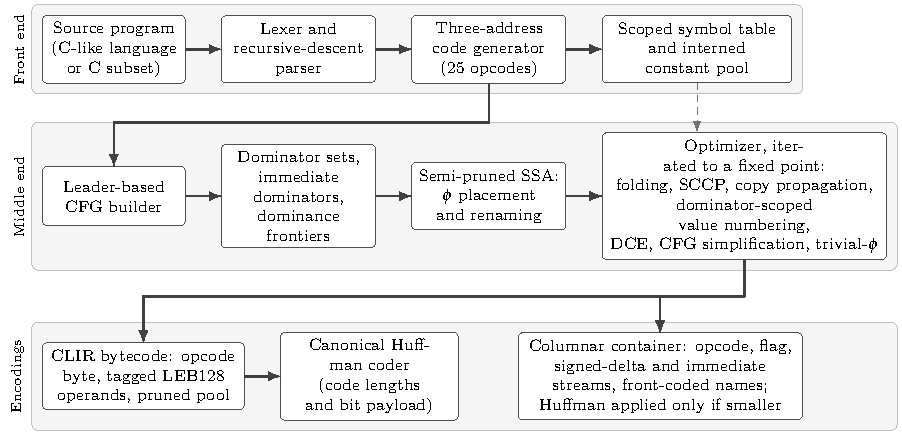
\includegraphics[width=\textwidth]{figures/fig_architecture.pdf}
\caption{Architecture of the proposed system (DCE: dead-code elimination). Solid arrows carry the program; the dashed arrow indicates that the constant pool and symbol names are also passed to the encoders.}
\label{fig:architecture}
\end{figure*}

The three tiers communicate only through plain data: an instruction list, a CFG with basic blocks, and byte strings. This makes each tier testable on its own, and it lets the evaluation scripts of Section~\ref{sec:results} observe every intermediate result. A command-line driver and a web front end, which draws the CFG and the dominator tree, sit on top of the same core.

\subsection{Detailed Methodology}

\subsubsection{Front end and three-address code}
The input language provides \texttt{int}, \texttt{float}, \texttt{string} and \texttt{bool} variables, arithmetic, relational and logical operators, \texttt{if}/\texttt{else}, \texttt{while} and \texttt{for} statements, nested blocks and a \texttt{print} statement. Simple C programs are accepted as well: preprocessor lines are skipped, the body of \texttt{int main()} is treated as a block, and \texttt{printf} is mapped to \texttt{print}. The TAC generator emits quadruples over 25 opcodes and loads every literal into a fresh temporary, so \texttt{int a = 10 + 20 * 3;} becomes six instructions.

\subsubsection{Control-flow graph and dominance}
Basic blocks start at the first instruction, at every jump target and after every jump or return; edges follow jumps, both outcomes of conditional jumps and fall-through. A block $d$ dominates $b$ if every path from the entry $r$ to $b$ passes through $d$. The dominator sets are the greatest fixed point of
\begin{equation}
\mathrm{Dom}(r)=\{r\},\qquad
\mathrm{Dom}(b)=\{b\}\cup\!\!\bigcap_{p\in \mathrm{pred}(b)}\!\!\mathrm{Dom}(p).
\label{eq:dom}
\end{equation}
The immediate dominator of $b\neq r$ is the strict dominator that all other strict dominators of $b$ dominate:
\begin{equation}
\begin{aligned}
\mathrm{idom}(b)&=d\in\mathrm{Dom}(b)\setminus\{b\}\\
&\text{such that}\ \ \mathrm{Dom}(b)\setminus\{b\}\subseteq \mathrm{Dom}(d).
\end{aligned}
\label{eq:idom}
\end{equation}
The dominance frontier of a block $x$ collects the join points where the dominance of $x$ ends:
\begin{equation}
\begin{aligned}
\mathrm{DF}(x)=\{\,y \mid{}& \exists p\in\mathrm{pred}(y):\ x\in\mathrm{Dom}(p)\\
&\wedge\ x\notin \mathrm{Dom}(y)\setminus\{y\}\,\}.
\end{aligned}
\label{eq:df}
\end{equation}
The implementation computes $\mathrm{DF}$ by walking up the dominator tree from each predecessor of a join block until the immediate dominator of the join block is reached~\cite{rastello2022ssa}.

\subsubsection{SSA construction}
A variable receives $\phi$-functions only if it is used in some block before being defined there, which yields semi-pruned SSA form. For such a variable $v$ with definition blocks $S_v$, the $\phi$-functions are placed on the iterated dominance frontier
\begin{equation}
\begin{aligned}
\mathrm{DF}^{+}(S_v)&=\lim_{i\to\infty}\mathrm{DF}_i,\qquad \mathrm{DF}_1=\mathrm{DF}(S_v),\\
\mathrm{DF}_{i+1}&=\mathrm{DF}(S_v\cup \mathrm{DF}_i).
\end{aligned}
\label{eq:idf}
\end{equation}
Variables are then renamed in a depth-first walk of the dominator tree, as listed in Algorithm~\ref{alg:ssa}. Fig.~\ref{fig:ssaexample} shows the result for benchmark S2, which contains an \texttt{if}/\texttt{else} diamond followed by a loop: three $\phi$-functions are inserted, one at the join of the diamond and two at the loop header.

\begin{algorithm}[t]
\caption{Semi-pruned SSA construction}
\label{alg:ssa}
\begin{algorithmic}[1]
\REQUIRE CFG $G$ with dominator tree and frontiers $\mathrm{DF}$
\ENSURE $G$ in SSA form
\STATE $\mathit{Glob}\gets$ variables used in a block before their definition there
\FORALL{$v\in\mathit{Glob}$}
  \STATE $W\gets S_v$ \COMMENT{blocks that define $v$}
  \WHILE{$W\neq\emptyset$}
    \STATE remove a block $x$ from $W$
    \FORALL{$y\in\mathrm{DF}(x)$ without a $\phi$ for $v$}
      \STATE insert $v\gets\phi(\,)$ after the labels of $y$
      \STATE \textbf{if} $y\notin S_v$ \textbf{then} add $y$ to $W$
    \ENDFOR
  \ENDWHILE
\ENDFOR
\STATE \textsc{Rename}$(r)$ \COMMENT{start at the entry block}
\STATE \textbf{procedure} \textsc{Rename}$(b)$
\STATE \quad give each $\phi$ and each definition in $b$ a new version $v_k$ and push it
\STATE \quad replace each use in $b$ by the top of its stack
\STATE \quad fill the $\phi$-arguments of every successor of $b$ for edge $(b,\cdot)$
\STATE \quad \textsc{Rename}$(c)$ for each child $c$ of $b$ in the dominator tree
\STATE \quad pop the versions pushed in $b$
\end{algorithmic}
\end{algorithm}

\begin{figure*}[!t]
\centering
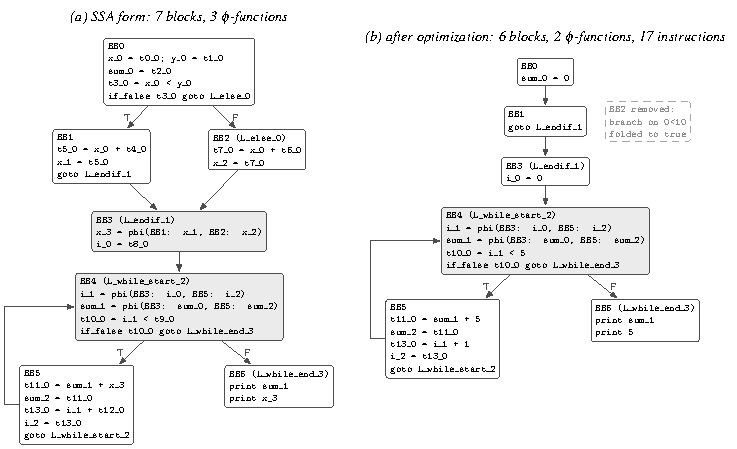
\includegraphics[width=0.94\textwidth]{figures/fig_ssa_example.pdf}
\caption{Worked example for benchmark S2. (a) SSA form produced by Algorithm~\ref{alg:ssa}; literal loads into temporaries (for example \texttt{t4\_0 = 5}) are omitted for space. (b) The same program after optimization: the branch on the constant condition $0<10$ is folded, BB2 becomes unreachable, the $\phi$-function for \texttt{x} becomes trivial, and the value 5 is propagated into the loop and the final \texttt{print}.}
\label{fig:ssaexample}
\end{figure*}

\subsubsection{Optimization passes}
The optimizer applies five passes in a loop until a round leaves the instruction count unchanged or ten rounds have run (Algorithm~\ref{alg:opt}). Constant folding rewrites an instruction whose operands are literals into a literal load,
\begin{equation}
\langle r\gets a\odot b\rangle,\ a,b\in\mathcal{L}\ \Longrightarrow\ \langle r\gets \mathrm{eval}_\odot(a,b)\rangle,
\label{eq:fold}
\end{equation}
where $\mathcal{L}$ is the set of literals; it also applies the identities $x+0=x$, $x\cdot1=x$, $x\cdot0=0$ and $x-0=x$, replaces operands defined as literals, and turns a conditional jump on a literal into a jump or a fall-through, removing the dead CFG edge and its $\phi$-arguments. Value numbering walks the dominator tree with a scoped table indexed by the key
\begin{equation}
\kappa(i)=\begin{cases}(\mathrm{op},\min(a,b),\max(a,b)) & \mathrm{op}\in\{+,\times,=,\neq\}\\ (\mathrm{op},a,b) & \text{otherwise,}\end{cases}
\label{eq:vn}
\end{equation}
and replaces a later instruction with the same key by a copy of the earlier result; entries are withdrawn when the walk leaves a subtree, so values never flow between sibling branches. Dead-code elimination repeatedly removes every instruction $i$ without side effects whose result is not used,
\begin{equation}
\mathrm{def}(i)\notin \bigcup_{j}\mathrm{uses}(j)\setminus\{\mathrm{def}(j)\mid j\text{ is a }\phi\}\ \Rightarrow\ \text{delete } i,
\label{eq:dce}
\end{equation}
where a $\phi$-function's use of its own result does not keep it alive. CFG simplification deletes unreachable blocks and stale $\phi$-arguments, and trivial-$\phi$ removal turns a $\phi$-function whose other arguments all name one value into a copy.

\begin{algorithm}[t]
\caption{Fixed-point driver of the optimizer}
\label{alg:opt}
\begin{algorithmic}[1]
\REQUIRE CFG $G$ in SSA form
\ENSURE optimized CFG $G$
\FOR{$k = 1$ \TO $10$}
  \STATE $n \gets$ number of instructions in $G$
  \STATE \textsc{FoldAndPropagate}$(G)$ \COMMENT{\eqref{eq:fold}; may delete edges}
  \STATE \textsc{ValueNumber}$(G)$ \COMMENT{\eqref{eq:vn}; dominator-tree walk}
  \STATE \textsc{EliminateDeadCode}$(G)$ \COMMENT{\eqref{eq:dce}}
  \STATE \textsc{PruneUnreachable}$(G)$
  \STATE \textsc{RemoveTrivialPhis}$(G)$
  \IF{number of instructions in $G = n$}
    \STATE \textbf{break}
  \ENDIF
\ENDFOR
\RETURN $G$
\end{algorithmic}
\end{algorithm}

\subsubsection{Encodings}
The optimized blocks are linearized in order and written as a \clir{} package, whose layout is drawn in Fig.~\ref{fig:layout}(a). Each instruction is one opcode byte followed by its operands as unsigned LEB128 integers, which store seven payload bits per byte. An operand $v$ whose binary form has $\beta(v)$ significant bits, with $\beta(0)=0$, therefore occupies
\begin{equation}
\ell(v)=\max\!\left(1,\left\lceil \beta(v)/7\right\rceil\right)\ \text{bytes}.
\label{eq:leb}
\end{equation}
Variable and label names are replaced by small integers in order of first appearance. With a constant pool of $p$ bytes and $m$ instructions whose operands are $v_{i,1},\dots,v_{i,k_i}$, the package size is
\begin{equation}
\begin{aligned}
|\clir{}| &= 5+\ell(p)+p+\ell(m)+\ell(\mathit{body})+\mathit{body},\\
\mathit{body} &= \sum_{i=1}^{m}\Big(1+\sum_{j=1}^{k_i}\ell(v_{i,j})\Big).
\end{aligned}
\label{eq:clir}
\end{equation}

The static Huffman stage (Fig.~\ref{fig:layout}(b)) counts the $k$ distinct byte values of the package and writes a header from which the decoder rebuilds the code tree: a 16-bit symbol count, each symbol with a 32-bit frequency, the 32-bit input length and a padding byte. For an input of $n$ bytes whose code gives length $\ell_s$ to a byte value $s$ of frequency $f_s$,
\begin{equation}
|H| = \underbrace{7 + 5k}_{\text{header}} + \left\lceil \frac{1}{8}\sum_{s} f_s\,\ell_s \right\rceil,
\qquad \sum_s f_s \ell_s \ge n\,\mathcal{H},
\label{eq:huff}
\end{equation}
where $\mathcal{H}$ is the empirical entropy of the input in bits per byte~\cite{moffat2019huffman}. Writing the payload as about $n\mathcal{H}/8$ bytes, coding saves space only when $n(1-\mathcal{H}/8)$ exceeds the header, which gives the break-even size
\begin{equation}
n^{\ast} \approx \frac{5k+7}{1-\mathcal{H}/8}.
\label{eq:breakeven}
\end{equation}

The columnar container (Fig.~\ref{fig:layout}(c)) splits the instructions into an opcode stream, a flag stream, a stream of backward distances from each use to its definition, and a stream of literals and labels stored as strings, followed by a front-coded table of source names. A leading flag byte records whether Huffman coding was applied, which is done only when it makes the container smaller. Algorithm~\ref{alg:enc} summarizes the encoding stage.

\begin{figure}[!t]
\centering
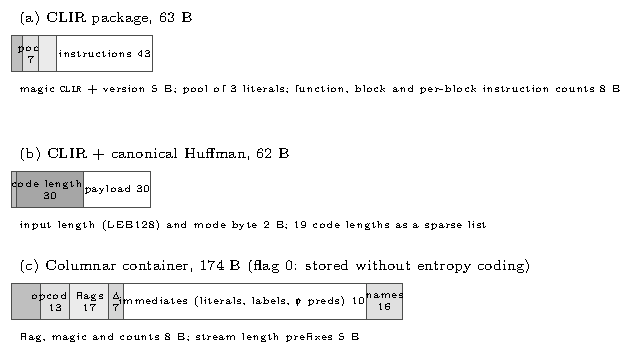
\includegraphics[width=\columnwidth]{figures/fig_layout.pdf}
\caption{Byte layout of the three encodings of benchmark S2, drawn to scale. The sizes are those measured in Section~\ref{sec:results}.}
\label{fig:layout}
\end{figure}

\begin{algorithm}[t]
\caption{Encoding with adaptive entropy coding}
\label{alg:enc}
\begin{algorithmic}[1]
\REQUIRE optimized instruction list $T^\ast$, constant pool $C$, names $N$
\ENSURE \clir{} package $B$, Huffman package $H$, container $Q$
\STATE $B\gets$ \texttt{"CLIR"} $\Vert$ version $\Vert$ LEB128$(|C|)$ $\Vert$ $C$
\FORALL{$t\in T^\ast$}
  \STATE append opcode byte of $t$ and LEB128 ids of its operands to $\mathit{body}$
\ENDFOR
\STATE $B\gets B\ \Vert$ LEB128$(|T^\ast|)$ $\Vert$ LEB128$(|\mathit{body}|)$ $\Vert$ $\mathit{body}$
\STATE $H\gets$ \textsc{HuffmanEncode}$(B)$
\STATE \textbf{assert} \textsc{HuffmanDecode}$(H)=B$
\STATE $S\gets$ opcode, flag, delta and immediate streams of $T^\ast$ and front-coded $N$
\STATE $h\gets$ \textsc{HuffmanEncode}$(S)$
\IF{$|h|<|S|$}
  \STATE $Q\gets \mathtt{0x01}\ \Vert\ h$
\ELSE
  \STATE $Q\gets \mathtt{0x00}\ \Vert\ S$
\ENDIF
\STATE \textbf{assert} decoding $Q$ reproduces the streams of $S$
\RETURN $B$, $H$, $Q$
\end{algorithmic}
\end{algorithm}

\subsection{Modules and Their Functions}
Fig.~\ref{fig:modules} lists the modules of the implementation and their main functions. The front end consists of the lexer, the parser, the TAC generator and the symbol and constant tables. The middle end consists of the CFG builder, the dominance analyzer, the SSA transformer and the optimizer. The back end holds the two encoding modules, and the interface layer consists of the command-line driver, an HTTP server with three endpoints and the browser front end. The evaluation scripts written for this article (Section~\ref{sec:results}) only read these modules and never modify them.

\begin{figure*}[!t]
\centering
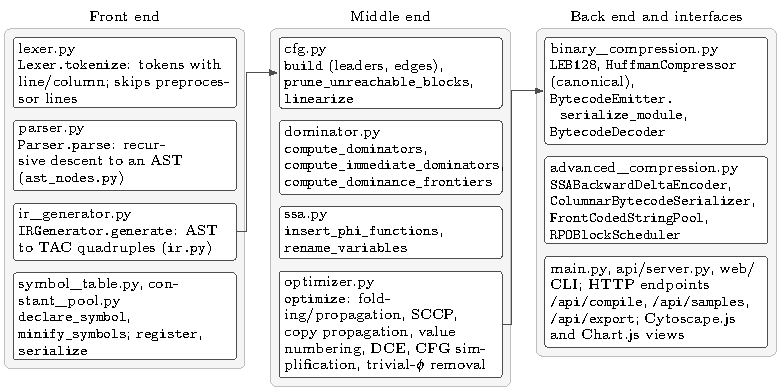
\includegraphics[width=0.9\textwidth]{figures/fig_modules.pdf}
\caption{Modules of the implementation and their main functions.}
\label{fig:modules}
\end{figure*}

%% Team contribution, as required by the course content template.
All four authors contributed equally to the design, implementation and evaluation of these modules, and every module was reviewed by at least one other team member.

\subsection{Flow Diagram}
Fig.~\ref{fig:flow} shows the processing flow for one program. A syntax error stops processing with the line and column of the offending token. Otherwise the program passes through TAC generation, CFG construction, dominance analysis and SSA construction. The optimizer then repeats its five passes while the instruction count keeps changing, for at most ten rounds. Finally, the encoder writes the \clir{} package and its Huffman-coded form, builds the columnar container, decides with one comparison whether that container is stored coded or raw, and verifies every round trip before reporting sizes.

\begin{figure}[!t]
\centering
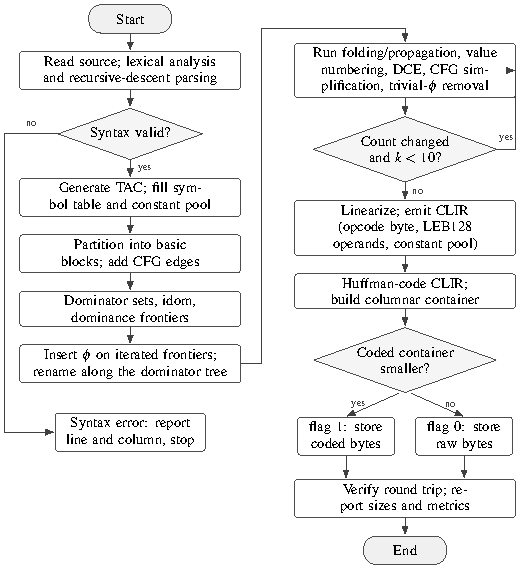
\includegraphics[width=\columnwidth]{figures/fig_flow.pdf}
\caption{Processing flow of the proposed system for one input program.}
\label{fig:flow}
\end{figure}

%% ===========================================================================
\section{Implementation and Result Analysis}
\label{sec:results}
%% ===========================================================================
\subsection{Tools, Configuration and Setup}
The system is written in Python and runs on the Python~3 standard library alone~\cite{python2024docs}; the web front end uses Cytoscape.js to draw graphs~\cite{franz2023cytoscape}. All measurements, except the comparison with Brotli and Zstandard, were taken with Python 3.13.16 on Linux 6.18 (x86-64) on a virtual machine with two cores of an Intel Xeon processor at 2.8~GHz. The comparison was run with Python 3.10.12 on Linux 6.8 (AArch64), calling the Brotli 1.0.9 and Zstandard 1.4.8 libraries through \texttt{ctypes}; on that machine the pipeline reproduced every size of the first machine byte for byte. A compilation is started with \texttt{python3 main.py --input benchmarks/<file>}, and the web front end with \texttt{python3 main.py --web --port 8000}.

The evaluation scripts in the directory \texttt{paper\_eval} are run in sequence, each with the command \texttt{python3} \texttt{paper\_eval/}\allowbreak\texttt{$\langle$name$\rangle$.py}: \texttt{measure}, \texttt{difftest} (once as released and once with the option \texttt{--cdiv}), \texttt{ablation}, \texttt{scaling}, \texttt{compare\_gp}, \texttt{derive}, \texttt{make\_tables} and \texttt{make\_figures}. They cross-check the pipeline in five ways: every printed percentage is recomputed; every \clir{} package is decoded by a parser written from Fig.~\ref{fig:layout}; every Huffman size is predicted with \eqref{eq:huff}; program behavior is compared by two reference interpreters, one for raw TAC and one for SSA graphs, which follow C's truncating division; and the 39 unit and regression tests of the core package are run, all of which pass. Fig.~\ref{fig:screenshot} shows the web front end of the implementation after compiling benchmark S2.

\begin{figure}[!t]
\centering
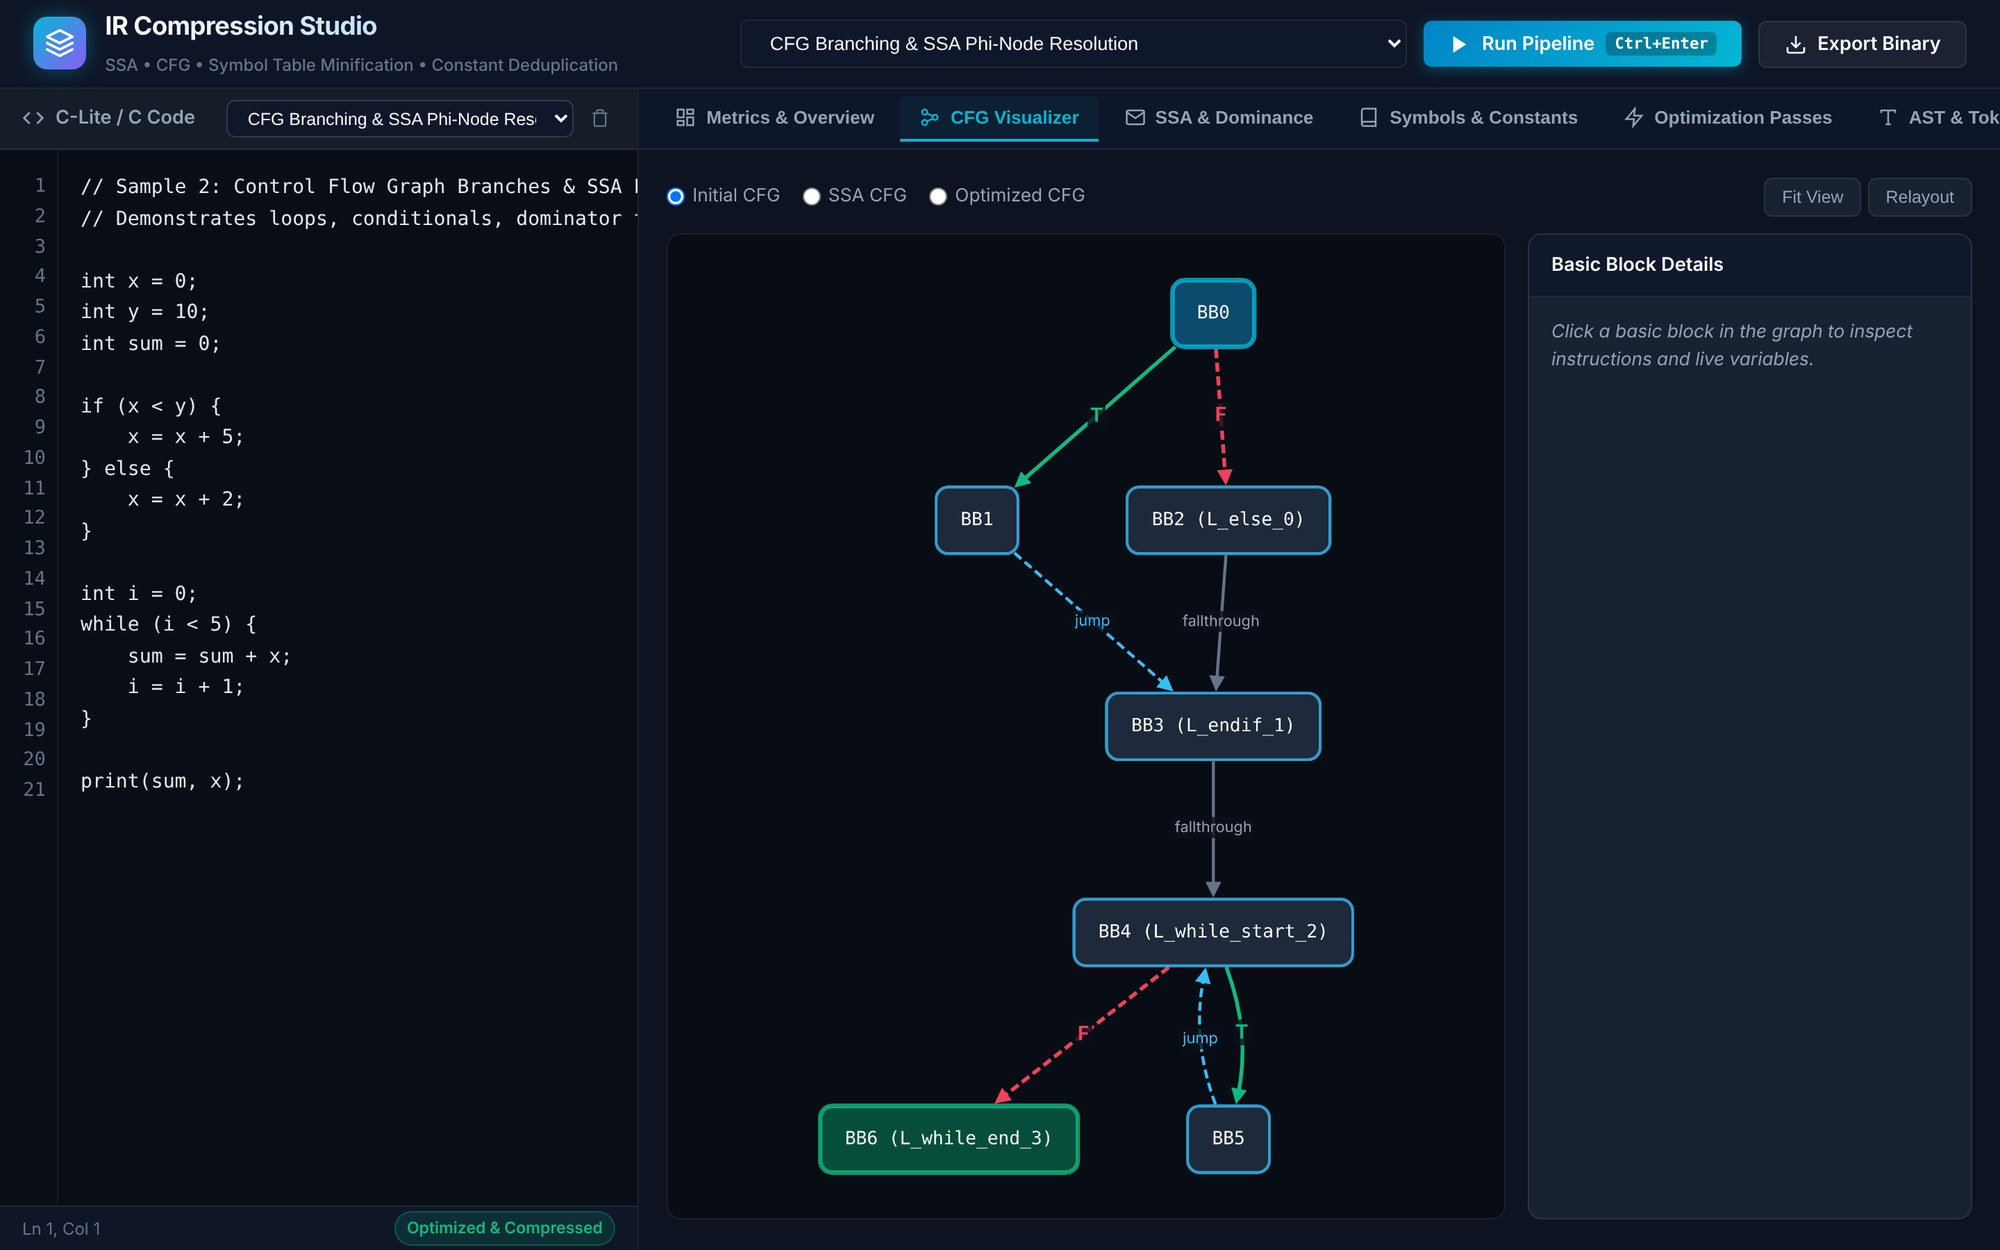
\includegraphics[width=\columnwidth]{figures/fig_screenshot.jpg}
\caption{Screenshot of the implementation: the web front end showing the source of benchmark S2 and its initial control-flow graph with true (T), false (F), jump and fall-through edges.}
\label{fig:screenshot}
\end{figure}

\subsection{Parameter Setup}
Table~\ref{tab:params} lists the parameters of the experiments. The seven bundled benchmarks are described in Table~\ref{tab:bench}. The synthetic programs come from a seeded generator that declares integer variables, assigns expressions with $+$, $-$, $\times$, $/$ and $\%$, and nests \texttt{if}/\texttt{else} statements and counter-controlled loops. Every variable is initialized and never shadowed, divisors are nonzero literals and loops run at most four times, so every program terminates without a run-time error.

\begin{table}[!t]
\centering
\caption{Parameter setup}
\label{tab:params}
\footnotesize
\setlength{\tabcolsep}{3pt}
\begin{tabular}{@{}p{30mm} p{51mm}@{}}
\toprule
Parameter & Value \\
\midrule
Bundled benchmarks & 7 programs, 326--539 bytes of source \\
Synthetic programs & 1264 in total: 200 (ablation), 64 (scaling: 8 size classes $\times$ 8 seeds), 1000 (differential testing); disjoint seeds \\
Program sizes & 4 to 512 top-level statements; loops of 1--4 iterations; nesting up to 3 levels \\
Optimizer & 5 passes, at most 10 rounds \\
Timing & median of 30 runs (benchmarks); minimum of 3 runs (synthetic) \\
Huffman alphabet & 256 byte values, 32-bit frequencies \\
Brotli & quality 11, window $2^{22}$, library 1.0.9 \\
Zstandard & level 19, library 1.4.8 \\
xz (LZMA2) & preset 9, \texttt{.xz} container \\
DEFLATE & level 9, raw stream \\
Platforms & Python 3.13.16, x86-64; Python 3.10.12, AArch64 \\
\bottomrule
\end{tabular}
\end{table}

\begin{table}[!t]
\centering
\caption{Bundled benchmarks. Instructions, blocks, edges and $\phi$-functions refer to the code before optimization.}
\label{tab:bench}
\footnotesize
\setlength{\tabcolsep}{3pt}
\begin{tabular}{@{}l l r r r r r@{}}
\toprule
ID & Focus & Source & TAC & Blocks & Edges & $\phi$ \\
 & & (B) & instr. & & & \\
\midrule
\rowsfrom{tables/tab_bench_rows.tex}
\bottomrule
\end{tabular}
\end{table}

\subsection{Performance Metrics}
Six metrics are used. For a quantity that falls from $a$ to $b$, the reduction is
\begin{equation}
R(a,b) = 100\,\frac{a-b}{a}\ \%,
\label{eq:red}
\end{equation}
which gives the instruction reduction when applied to instruction counts and the size reduction when applied to bytes. The encoding density is the number of bits spent per instruction,
\begin{equation}
\rho=\frac{8\,|X|}{N},
\label{eq:density}
\end{equation}
for a representation $X$ of $N$ instructions. The compilation throughput is $\Theta=n/t$ instructions per second for a program of $n$ raw instructions compiled in time $t$, and the entropy-coding overhead is the share $(7+5k)/|H|$ of the header in \eqref{eq:huff}. Correctness is measured by the agreement rate
\begin{equation}
A=100\,\frac{|\{P:\ \mathrm{Obs}(T_P^\ast)=\mathrm{Obs}(T_P)\}|}{|\{P\}|}\ \%
\label{eq:agree}
\end{equation}
over a set of programs $P$. \emph{Raw TAC text} denotes the unoptimized instructions, one per line, in UTF-8; it is the baseline that the tool itself reports against.

\subsection{Results}

\subsubsection{Instruction reduction}
Table~\ref{tab:opt} and Fig.~\ref{fig:reduction} show the instruction counts before and after optimization. The reduction ranges from 18.5\% for S5 to 89.3\% for S4, with a mean of 58.4\%. Programs whose values are all known at compile time (S1, S3 and S4) shrink the most, because folding turns every computation into a literal and dead-code elimination removes the literal loads. S5, an iterative Fibonacci loop, keeps most of its code because its loop-carried values reach the loop through $\phi$-functions, through which the folder does not propagate. Value numbering found nothing to remove in any benchmark, since folding had already turned the repeated expressions of S3 into constants.

\begin{table}[!t]
\centering
\caption{Effect of optimization on the benchmarks: instruction counts, reduction $R$ (\%), blocks after optimization, and the work done by each pass (VN: value numbering)}
\label{tab:opt}
\footnotesize
\setlength{\tabcolsep}{2.6pt}
\begin{tabular}{@{}l r r r r r r r r r@{}}
\toprule
ID & TAC & Opt. & Red. & Blocks & Folds & Prop. & Dead & Dead & VN \\
 & & & (\%) & & & & instr. & blocks & hits \\
\midrule
\rowsfrom{tables/tab_opt_rows.tex}
\bottomrule
\end{tabular}
\end{table}

\begin{figure}[!t]
\centering
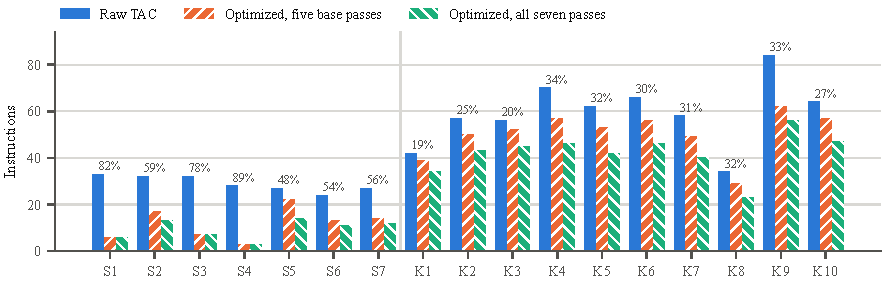
\includegraphics[width=\columnwidth]{figures/fig_reduction.pdf}
\caption{Instructions before and after optimization; the label gives the reduction $R$.}
\label{fig:reduction}
\end{figure}

Fig.~\ref{fig:ablation} explains where the reduction comes from, using 200 synthetic programs with one pass disabled at a time. With all passes, the 68\,630 raw instructions fall to 30\,179, a reduction of 56.0\%. Disabling dead-code elimination increases the result by 118.7\% and disabling folding and propagation by 86.0\%; the two passes work together, because folding produces dead literal loads that only dead-code elimination removes. Value numbering replaced 77 expressions in 57 of the programs, but turning it off changed the total by only five instructions, because a replaced expression becomes a copy and there is no copy propagation to remove it.

\begin{figure}[!t]
\centering
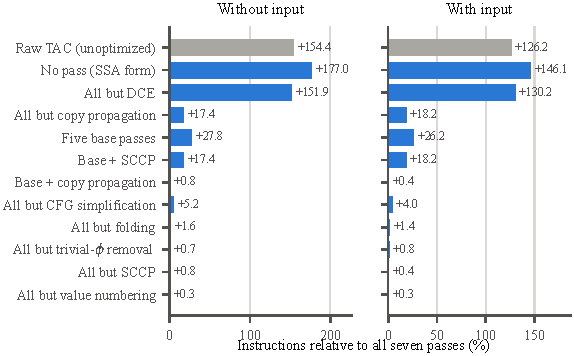
\includegraphics[width=\columnwidth]{figures/fig_ablation.pdf}
\caption{Per-pass ablation over 200 synthetic programs: total instructions after optimization with one pass disabled, relative to all passes enabled. The gray bar is the unoptimized TAC.}
\label{fig:ablation}
\end{figure}

\subsubsection{Size reduction and comparison with existing works}
Table~\ref{tab:size} and Fig.~\ref{fig:bench} give the size of every representation. The \clir{} package of the optimized program is 68.7\% to 87.8\% smaller than the raw TAC text. For comparison with existing approaches, we compressed the raw TAC text with three widely used general-purpose compressors: Brotli~\cite{alakuijala2019brotli}, Zstandard~\cite{collet2021zstd} and xz~\cite{tukaani2024xz}. Table~\ref{tab:compare} and Fig.~\ref{fig:compare} show that the \clir{} package, without any entropy coder, is 37.3\% to 75.4\% smaller than the best of the three on every benchmark. On the 64 synthetic programs of the scaling study it was smaller than the best of the three in all 64 cases, by 14.7\% to 70.1\%. Applying Brotli to the \clir{} package reduces it further, for example from 104 to 83 bytes for S5.

The justification is that the two stages remove different kinds of redundancy. The compressors find repeated byte strings but must keep every instruction, whereas the optimizer removes instructions and the bytecode replaces names and literals by one-byte indices. Two caveats apply. First, literal operands that propagation places directly into instructions are encoded as register indices whose values are not written to the package, so a decoder needs a small side table that is not counted. Second, the constant pool is written as built by the front end: in S4 it takes 47 of the 61 bytes although no remaining instruction refers to it.

\begin{table*}[!t]
\centering
\caption{Encoded size in bytes. \clir{} is shown as total (constant pool/instruction body); Huffman as total (frequency table/payload). The entropy bound is $n\mathcal{H}/8$ for the \clir{} package. ``Columnar'' includes its one-byte flag. The last three columns apply raw DEFLATE (level 9) to the raw TAC text, to the optimized text and to the \clir{} package.}
\label{tab:size}
\footnotesize
\setlength{\tabcolsep}{4.2pt}
\begin{tabular}{@{}l r r r r r r r r r r@{}}
\toprule
ID & Raw TAC & Optimized & \clir{} & \clir{} vs.\ raw & \clir{}+Huffman & Entropy & Columnar & DEFLATE & DEFLATE & DEFLATE \\
 & text & text & (pool/body) & text, $R$ (\%) & (table/payload) & bound & & (raw text) & (opt.\ text) & (\clir{}) \\
\midrule
\rowsfrom{tables/tab_size_rows.tex}
\bottomrule
\end{tabular}
\end{table*}

\begin{figure*}[!t]
\centering
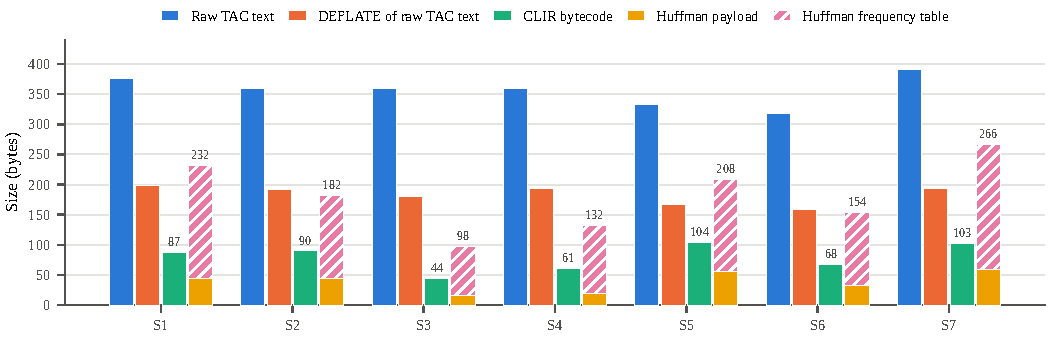
\includegraphics[width=\textwidth]{figures/fig_benchmark_sizes.pdf}
\caption{Encoded size of the seven benchmarks. The Huffman bar is split into its frequency table (hatched) and its payload; the number above it is the total. The number above the \clir{} bar is its size.}
\label{fig:bench}
\end{figure*}

\begin{table}[!t]
\centering
\caption{Comparison with existing compressors applied to the raw TAC text (bytes). $R$ is the reduction of \clir{} relative to the best of Brotli, Zstandard and xz.}
\label{tab:compare}
\footnotesize
\setlength{\tabcolsep}{2.6pt}
\begin{tabular}{@{}l r r r r r r r@{}}
\toprule
ID & Raw & Brotli & Zstd & xz & \clir{} & $R$ & \clir{} \\
 & text & \cite{alakuijala2019brotli} & \cite{collet2021zstd} & \cite{tukaani2024xz} & & (\%) & +Brotli \\
\midrule
\rowsfrom{tables/tab_compare_rows.tex}
\bottomrule
\end{tabular}
\end{table}

\begin{figure*}[!t]
\centering
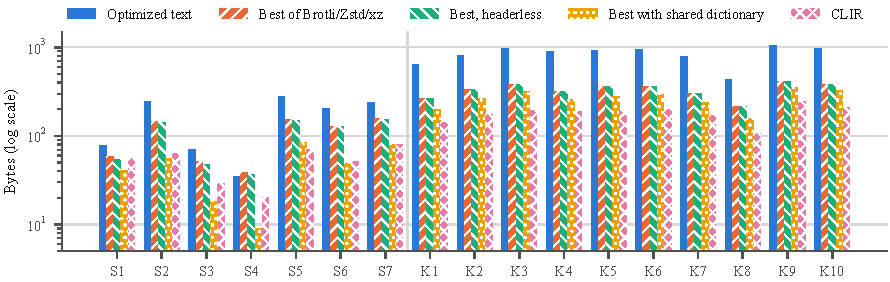
\includegraphics[width=\textwidth]{figures/fig_compare.pdf}
\caption{Comparison with existing general-purpose compressors applied to the raw TAC text. The proposed \clir{} encoding (labeled) is smaller on every benchmark; applying Brotli to \clir{} shrinks it further.}
\label{fig:compare}
\end{figure*}

\subsubsection{Encoding density}
Fig.~\ref{fig:density} expresses the same sizes per instruction with \eqref{eq:density}. The raw TAC text spends 90.0 to 115.9 bits per instruction. The \clir{} instruction body spends 16.0 to 26.9 bits per optimized instruction: 16 bits is one opcode byte plus one operand byte, and loops and $\phi$-functions add operands. Counted against the original instructions, the whole \clir{} package costs 11.0 to 30.8 bits per raw instruction, because optimization has removed many of them.

\begin{figure}[!t]
\centering
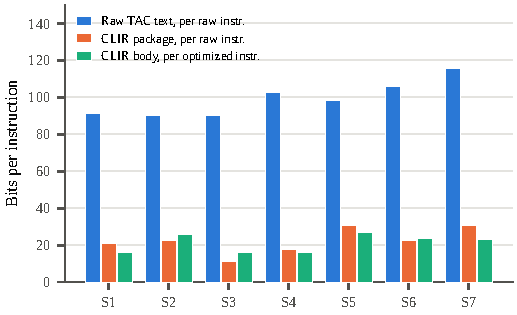
\includegraphics[width=\columnwidth]{figures/fig_density.pdf}
\caption{Encoding density in bits per instruction, from \eqref{eq:density}.}
\label{fig:density}
\end{figure}

\subsubsection{Entropy-coding overhead}
The static Huffman stage made every benchmark 2.0 to 2.7 times larger than its \clir{} input. Its payload is within 1.5 bytes of the entropy bound, but the frequency table takes 73.1\% to 84.8\% of the output (Table~\ref{tab:size}). Fig.~\ref{fig:scaling} shows where the stage starts to help. Across the 64 synthetic programs, Huffman coding was larger than its input for every package of up to 5691 bytes and smaller for every package of 5736 bytes or more. In 32 of the programs all 256 byte values occur, so the header is fixed at 1287 bytes, and the entropy lies between 6.11 and 6.57 bits per byte. With $\mathcal{H}\approx6.2$, \eqref{eq:breakeven} predicts $n^{\ast}\approx5.7$ kB, which matches the observed threshold; applied program by program, it classifies 63 of the 64 programs correctly. In the largest size class, with a median of 8034 raw instructions, Huffman coding saved 12.2\% and DEFLATE applied to \clir{} saved 21.4\%. The columnar container was larger than \clir{} in every size class.

\begin{figure}[!t]
\centering
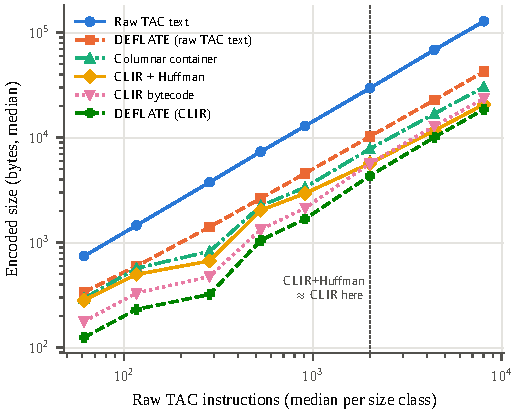
\includegraphics[width=\columnwidth]{figures/fig_scaling.pdf}
\caption{Median encoded size against median program size for eight size classes of synthetic programs (eight programs each). The dotted line marks the class in which Huffman coding first produced output smaller than its \clir{} input.}
\label{fig:scaling}
\end{figure}

\subsubsection{Latency and throughput}
Table~\ref{tab:time} breaks the compilation time of each benchmark down by stage. The complete pipeline takes between 1.48 and 3.19~ms per benchmark, of which the optimizer takes 9.9\% to 25.4\%. Fig.~\ref{fig:throughput} shows the time for all 64 synthetic programs. A least-squares fit on the logarithms gives an exponent of 1.14, so growth is slightly faster than linear. The throughput ranges from 4771 to 21\,289 raw instructions per second. In the three largest programs we profiled, one from each of the three largest size classes, the optimizer was the most expensive stage, with 37.4\% to 46.9\% of the time, because every round recomputes the dominator tree for value numbering with the fixed point of \eqref{eq:dom}.

\begin{table}[!t]
\centering
\caption{Median running time per stage in milliseconds (30 runs)}
\label{tab:time}
\footnotesize
\setlength{\tabcolsep}{2.8pt}
\begin{tabular}{@{}l r r r r r r r r@{}}
\toprule
ID & Front & TAC & CFG, & SSA & Opt. & \clir{}, & Colum- & Total \\
 & end & & dom. & & & Huff. & nar & \\
\midrule
\rowsfrom{tables/tab_time_rows.tex}
\bottomrule
\end{tabular}
\end{table}

\begin{figure}[!t]
\centering
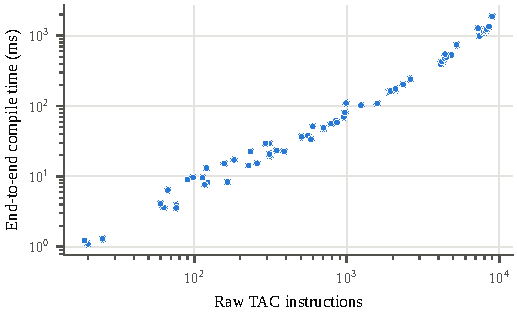
\includegraphics[width=\columnwidth]{figures/fig_throughput.pdf}
\caption{End-to-end compilation time of the 64 synthetic programs (minimum of three runs; both axes logarithmic).}
\label{fig:throughput}
\end{figure}

\subsubsection{Correctness}
On the seven benchmarks the raw TAC, the SSA form and the optimized form printed identical values, which also match the values we computed by hand. Every \clir{} package decoded to the expected instruction sequence, and every Huffman package matched \eqref{eq:huff} exactly and decompressed to its input. Table~\ref{tab:diff} summarizes differential testing on 1000 random programs with between 15 and 1173 raw instructions each, 347\,497 in total. The SSA form agreed with the raw TAC on all of them. The optimized form disagreed on 214 programs, an agreement rate of 78.6\%.

Every one of these divergences disappears when both interpreters use floor division. The folder evaluates integer \texttt{/} and \texttt{\%} with Python's floor semantics, whereas C truncates toward zero, so an expression whose value is $-31$ reduced modulo 1000 folds to $969$ instead of $-31$. With a folder that truncates, all 1000 programs agree. The high rate of divergence is a property of our generator, which often applies \texttt{\%} to negative values. The columnar container passes its own round-trip check, but 7 of the 14 $\phi$-arguments in S2, S5, S6 and S7 refer to definitions that come later in the linear order. The backward-distance scheme stores 0 for them, so those arguments cannot be recovered from the container.

\begin{table}[!t]
\centering
\caption{Differential testing on 1000 random programs: programs whose optimized form printed the same values as the raw TAC}
\label{tab:diff}
\footnotesize
\setlength{\tabcolsep}{3pt}
\begin{tabular}{@{}l r r r r@{}}
\toprule
Folder variant & Programs & Agree & Differ: & Differ: \\
 & & & division & other \\
\midrule
\rowsfrom{tables/tab_diff_rows.tex}
\bottomrule
\end{tabular}
\end{table}

\subsubsection{Threats to validity}
The benchmarks are small and were written to illustrate the passes, and the synthetic programs have no input, so in principle all their values are compile-time constants; real programs with input and function calls would leave less to folding. Percentages depend on the baseline, which is why the raw text, the optimized text and three compressors are all reported. The reference interpreters were written for this study and could share a misconception with the pipeline, although they agree with the hand-computed outputs of all seven benchmarks.

%% ===========================================================================
\section{Conclusion and Scope for Future Work}
\label{sec:conclusion}
%% ===========================================================================
This article presented an SSA-based pipeline that compacts three-address code by optimizing it first and encoding it second, and checked every reported number independently.

Existing methodologies either shrink native code inside large production compilers or compress intermediate code as an opaque file with general-purpose compressors.

The proposed method removes instructions with five SSA passes and writes the rest with one opcode byte and LEB128 operands. Its advantage is that each stage is measured separately and behavior is verified.

The system was implemented in Python with a Cytoscape.js web front end, and evaluated with independent decoders, reference interpreters and differential testing.

Optimization removed 18.5\% to 89.3\% of the instructions of seven benchmarks. The \clir{} bytecode was 68.7\% to 87.8\% smaller than the raw text and 37.3\% to 75.4\% smaller than Brotli, Zstandard or xz applied to that text. Static Huffman coding paid off only above about 5.7~kB, as the break-even model predicts. Differential testing on 1000 programs found one folding defect and confirmed its fix.

Future work will add copy propagation, so that value numbering can remove instructions, and constant propagation through $\phi$-functions. The bytecode will be made self-describing, with a pruned constant pool and a table for literal operands. The frequency-table coder will be replaced by a canonical or pre-trained entropy coder. The columnar container will be extended to represent loop-carried $\phi$-arguments. Finally, the evaluation will move to programs translated from an established C benchmark suite.

%% ===========================================================================
\begin{thebibliography}{00}

\bibitem{bauwens2020ota}
Bauwens, Jan, Peter Ruckebusch, Spilios Giannoulis, Ingrid Moerman, and Eli De Poorter. (2020) ``Over-the-air software updates in the Internet of Things: an overview of key principles.'' \emph{IEEE Communications Magazine} \textbf{58} (\textbf{2}): 35--41.

\bibitem{w3c2019wasm}
World Wide Web Consortium (W3C). (2019) ``WebAssembly core specification.'' W3C Recommendation, 5 December 2019. \url{https://www.w3.org/TR/wasm-core-1/}

\bibitem{jangda2019wasm}
Jangda, Abhinav, Bobby Powers, Emery D. Berger, and Arjun Guha. (2019) ``Not so fast: analyzing the performance of WebAssembly vs. native code.'' In \emph{Proceedings of the 2019 USENIX Annual Technical Conference (USENIX ATC '19)}, 107--120.

\bibitem{lattner2021mlir}
Lattner, Chris, Mehdi Amini, Uday Bondhugula, Albert Cohen, Andy Davis, Jacques Pienaar, River Riddle, Tatiana Shpeisman, Nicolas Vasilache, and Oleksandr Zinenko. (2021) ``MLIR: scaling compiler infrastructure for domain specific computation.'' In \emph{Proceedings of the 2021 IEEE/ACM International Symposium on Code Generation and Optimization (CGO)}, 2--14.

\bibitem{rastello2022ssa}
Rastello, Fabrice, and Florent Bouchez Tichadou (eds). (2022) \emph{SSA-based Compiler Design}. Cham, Springer.

\bibitem{cooper2022eac}
Cooper, Keith D., and Linda Torczon. (2022) \emph{Engineering a Compiler}, 3rd edition. Cambridge, MA, Morgan Kaufmann.

\bibitem{wang2018ml}
Wang, Zheng, and Michael O'Boyle. (2018) ``Machine learning in compiler optimization.'' \emph{Proceedings of the IEEE} \textbf{106} (\textbf{11}): 1879--1901.

\bibitem{ashouri2018autotuning}
Ashouri, Amir H., William Killian, John Cavazos, Gianluca Palermo, and Cristina Silvano. (2018) ``A survey on compiler autotuning using machine learning.'' \emph{ACM Computing Surveys} \textbf{51} (\textbf{5}): 1--42.

\bibitem{moffat2019huffman}
Moffat, Alistair. (2019) ``Huffman coding.'' \emph{ACM Computing Surveys} \textbf{52} (\textbf{4}): 1--35.

\bibitem{rocha2020salssa}
Rocha, Rodrigo C. O., Pavlos Petoumenos, Zheng Wang, Murray Cole, and Hugh Leather. (2020) ``Effective function merging in the SSA form.'' In \emph{Proceedings of the 41st ACM SIGPLAN Conference on Programming Language Design and Implementation (PLDI)}, 854--868.

\bibitem{rocha2021hyfm}
Rocha, Rodrigo C. O., Pavlos Petoumenos, Zheng Wang, Murray Cole, Kim Hazelwood, and Hugh Leather. (2021) ``HyFM: function merging for free.'' In \emph{Proceedings of the 22nd ACM SIGPLAN/SIGBED International Conference on Languages, Compilers, and Tools for Embedded Systems (LCTES)}, 110--121.

\bibitem{rocha2022rolag}
Rocha, Rodrigo C. O., Pavlos Petoumenos, Bj\"orn Franke, Pramod Bhatotia, and Michael O'Boyle. (2022) ``Loop rolling for code size reduction.'' In \emph{Proceedings of the 2022 IEEE/ACM International Symposium on Code Generation and Optimization (CGO)}, 217--229.

\bibitem{damasio2021inlining}
Dam\'asio, Tha\'is, Vin\'icius Pacheco, Fabr\'icio Goes, Fernando Pereira, and Rodrigo Rocha. (2021) ``Inlining for code size reduction.'' In \emph{Proceedings of the 25th Brazilian Symposium on Programming Languages (SBLP)}, 17--24.

\bibitem{theodoridis2022inlining}
Theodoridis, Theodoros, Tobias Grosser, and Zhendong Su. (2022) ``Understanding and exploiting optimal function inlining.'' In \emph{Proceedings of the 27th ACM International Conference on Architectural Support for Programming Languages and Operating Systems (ASPLOS)}, 977--989.

\bibitem{chabbi2021ios}
Chabbi, Milind, Jin Lin, and Raj Barik. (2021) ``An experience with code-size optimization for production iOS mobile applications.'' In \emph{Proceedings of the 2021 IEEE/ACM International Symposium on Code Generation and Optimization (CGO)}, 363--377.

\bibitem{trofin2021mlgo}
Trofin, Mircea, Yundi Qian, Eugene Brevdo, Zinan Lin, Krzysztof Choromanski, and David Li. (2021) ``MLGO: a machine learning guided compiler optimizations framework.'' \emph{arXiv preprint} arXiv:2101.04808.

\bibitem{jain2022posetrl}
Jain, Shalini, Yashas Andaluri, S. VenkataKeerthy, and Ramakrishna Upadrasta. (2022) ``POSET-RL: phase ordering for optimizing size and execution time using reinforcement learning.'' In \emph{Proceedings of the 2022 IEEE International Symposium on Performance Analysis of Systems and Software (ISPASS)}, 121--131.

\bibitem{cummins2023llm}
Cummins, Chris, Volker Seeker, Dejan Grubisic, Mostafa Elhoushi, Youwei Liang, Baptiste Roziere, Jonas Gehring, Fabian Gloeckle, Kim Hazelwood, Gabriel Synnaeve, and Hugh Leather. (2023) ``Large language models for compiler optimization.'' \emph{arXiv preprint} arXiv:2309.07062.

\bibitem{cummins2021compilergym}
Cummins, Chris, Bram Wasti, Jiadong Guo, Brandon Cui, Jason Ansel, Sahir Gomez, Somya Jain, Jia Liu, Olivier Teytaud, Benoit Steiner, Yuandong Tian, and Hugh Leather. (2021) ``CompilerGym: robust, performant compiler optimization environments for AI research.'' \emph{arXiv preprint} arXiv:2109.08267.

\bibitem{cummins2021programl}
Cummins, Chris, Zacharias V. Fisches, Tal Ben-Nun, Torsten Hoefler, Michael F. P. O'Boyle, and Hugh Leather. (2021) ``ProGraML: a graph-based program representation for data flow analysis and compiler optimizations.'' In \emph{Proceedings of the 38th International Conference on Machine Learning (ICML)}, PMLR \textbf{139}: 2244--2253.

\bibitem{chen2020testing}
Chen, Junjie, Jibesh Patra, Michael Pradel, Yingfei Xiong, Hongyu Zhang, Dan Hao, and Lu Zhang. (2020) ``A survey of compiler testing.'' \emph{ACM Computing Surveys} \textbf{53} (\textbf{1}): 1--36.

\bibitem{hilbig2021wasm}
Hilbig, Aaron, Daniel Lehmann, and Michael Pradel. (2021) ``An empirical study of real-world WebAssembly binaries: security, languages, use cases.'' In \emph{Proceedings of the Web Conference 2021 (WWW '21)}, 2696--2708.

\bibitem{cabrera2020superopt}
Cabrera Arteaga, Javier, Shrinish Donde, Jian Gu, Orestis Floros, Lucas Satabin, Benoit Baudry, and Martin Monperrus. (2020) ``Superoptimization of WebAssembly bytecode.'' \emph{arXiv preprint} arXiv:2002.10213.

\bibitem{lopes2021alive2}
Lopes, Nuno P., Juneyoung Lee, Chung-Kil Hur, Zhengyang Liu, and John Regehr. (2021) ``Alive2: bounded translation validation for LLVM.'' In \emph{Proceedings of the 42nd ACM SIGPLAN International Conference on Programming Language Design and Implementation (PLDI)}, 65--79.

\bibitem{livinskii2020yarpgen}
Livinskii, Vsevolod, Dmitry Babokin, and John Regehr. (2020) ``Random testing for C and C++ compilers with YARPGen.'' \emph{Proceedings of the ACM on Programming Languages} \textbf{4} (\textbf{OOPSLA}): 196:1--196:25.

\bibitem{python2024docs}
Python Software Foundation. (2024) ``Python 3.13 documentation.'' \url{https://docs.python.org/3.13/}

\bibitem{franz2023cytoscape}
Franz, Max, Christian T. Lopes, Dylan Fong, Mike Kucera, Manfred Cheung, Metin Can Siper, Gerardo Huck, Dong Yue, Onur Sumer, and Gary D. Bader. (2023) ``Cytoscape.js 2023 update: a graph theory library for visualization and analysis.'' \emph{Bioinformatics} \textbf{39} (\textbf{1}): btad031.

\bibitem{alakuijala2019brotli}
Alakuijala, Jyrki, Andrea Farruggia, Paolo Ferragina, Eugene Kliuchnikov, Robert Obryk, Zoltan Szabadka, and Lode Vandevenne. (2019) ``Brotli: a general-purpose data compressor.'' \emph{ACM Transactions on Information Systems} \textbf{37} (\textbf{1}): 1--30.

\bibitem{collet2021zstd}
Collet, Yann, and Murray S. Kucherawy. (2021) ``Zstandard compression and the application/zstd media type.'' RFC 8878, Internet Engineering Task Force. \url{https://www.rfc-editor.org/rfc/rfc8878}

\bibitem{tukaani2024xz}
Tukaani Project. (2024) ``XZ Utils.'' \url{https://github.com/tukaani-project/xz}

\end{thebibliography}

%% ---------------------------------------------------------------------------
%% End sections required by the course content template
%% ---------------------------------------------------------------------------
\section*{Author Contributions}
All authors contributed equally to the design, implementation and writing of this work, and all authors read and approved the final manuscript.

\section*{Acknowledgements}
%% IEEE Access requires AI-assisted text to be disclosed here, naming the AI
%% system and what it was used for. Keep this statement accurate.
The compiler evaluated in this article was designed and implemented by the authors. The authors used the AI assistant Claude (Anthropic) to draft the manuscript text and to write the evaluation scripts and figures of Section~\ref{sec:results}. All such material was checked against the measured results and revised by the authors, who take full responsibility for the content of this article.

\section*{Funding}
This work received no external funding.

\section*{Competing Interests}
The authors declare no competing interests.

\section*{Data and Code Availability}
The source code of the compiler is available at \url{https://github.com/rishbCLN/compiler_project}. The evaluation scripts that produce every table and figure in this article are available from the corresponding author on reasonable request.

%% Author biographies with photographs (required by IEEE Access for journal
%% submission) are omitted: the course content template does not ask for them.

\EOD

\end{document}
